\documentclass{article}
\usepackage{graphicx} % For including images
\usepackage{titling}  % For custom title page
\usepackage{circuitikz}
\usepackage{amsmath}
\usepackage{amssymb}
\usepackage{booktabs,tabu}
\usepackage[all, cmtip]{xy}
\newcommand{\ohm}{\Omega}
% Set up title and author
\title{Experiment 6: Sampling}
\author{Samyak Sheersh,Souhardya Bose,Aryam Shankar}
\date{21 October 2024}
\newcommand{\subtitle}[1]{%
  \posttitle{%
    \par\end{center}
    \begin{center}\large#1\end{center}
    \vskip0.5em}%
}

\begin{document}

% Custom title page
\begin{titlepage}
    \centering
    
\includegraphics[width=0.2\textwidth]{KGP_logo.png}\par\vspace{1cm}
    {\scshape\LARGE Department of Electronics and Electrical Communication Engineering, IIT Kharagpur\par}
    \vspace{1cm}
    {\huge\bfseries Experiment 6: Sampling\par}
    \vspace{1.5cm}
    {\Large\itshape Samyak Sheersh,Souhardya Bose,Aryam Shankar\par}
    \vfill
    % Identifying information at the bottom
    {\large Roll Numbers: 22EC30045, 21EE10097, 22EC3FP37\par}
    {\large Group Number: 12\par}
    \vfill
    {\large 21 October 2024\par}
\end{titlepage}


\section{Introduction}
\subsection{Objectives}
\begin{enumerate}
  \item To sample and hold a given input signal
  \item To generate a Pulse Amplitude Modulated(PAM) signal
\end{enumerate}
\section{Instruments and Materials Used}
\begin{enumerate}
  \item RIGOL Signal Generator
  \item ScientiFIC SMO10C Digital Signal Oscilloscope
  \item +12V, -12V DC source and ground
  \item Resistors
  \item Capacitors
  \item Diodes
  \item Breadboard
  \item Connecting wires
  \item JFET
  \item Potentiometer
\end{enumerate}
\section{Theory}

A sample and hold circuit is frequently used in analog-to-digital conversion system, and it holde the value for a certain period allowing further processing to happen, and is essential to digitize and store signals. In relation to this circuit, we define two terms:
\begin{enumerate}
  \item Aperture time: The time during which the sampling occurs. Ideally we want it to be zero i.e store instantaneous precise values, but we strive to keep it as short as possible.
  \item Hold time: The duration in which the sampled value is held constant by the capacitor. 
\end{enumerate}

A Pulse Amplitude Modulation(PAM) is a form of signal modulation where the amplitude of a series of pulses is varied according to the instantaneous values of the signal
\clearpage
\section{Circuit Diagram}
\begin{figure}[!ht]
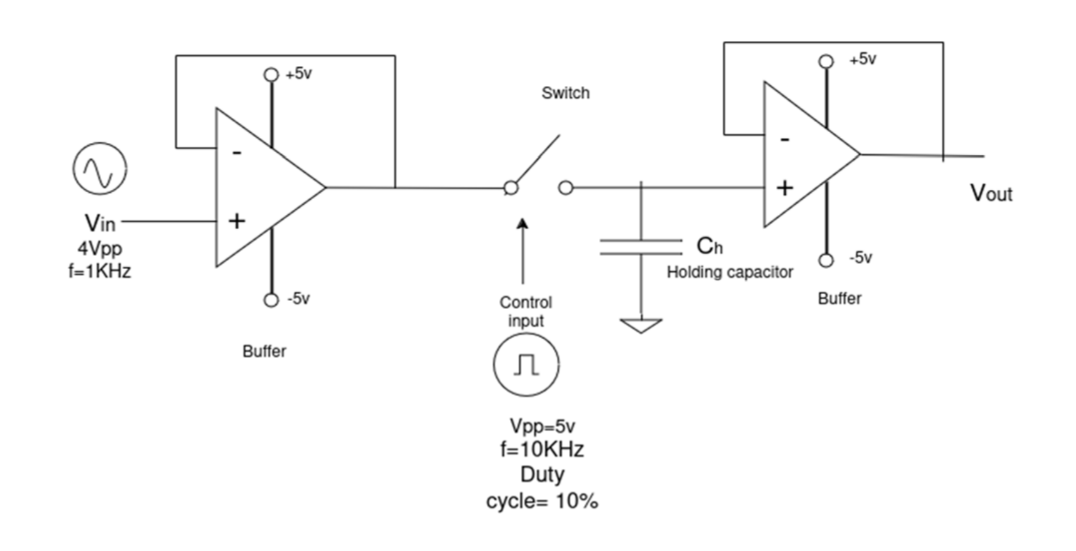
\includegraphics[width=\textwidth]{Sample_and_hold.png}
\caption{A sample and hold circuit diagram}
\label{fig:sample_and_hold}
\end{figure}

\begin{figure}[!ht]
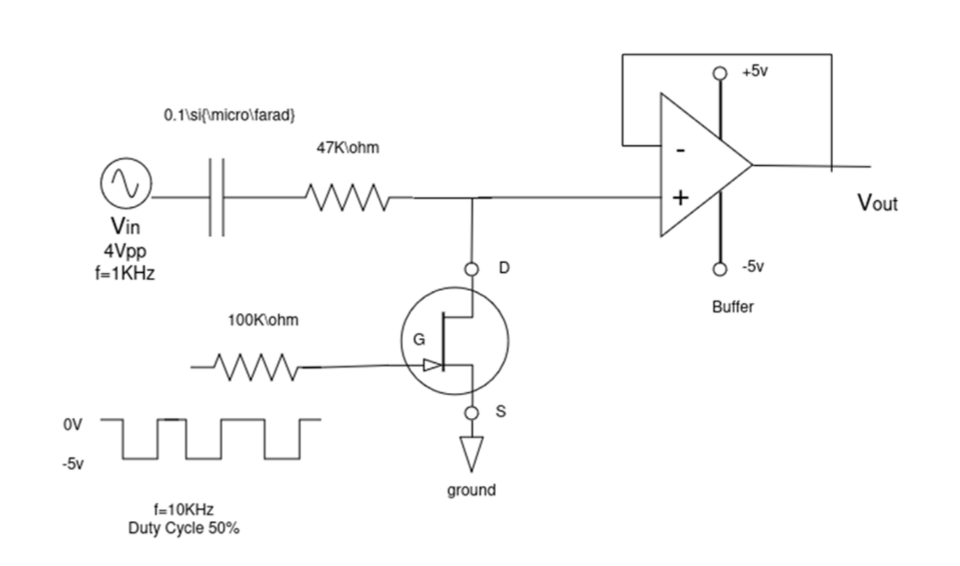
\includegraphics[width=\textwidth]{PAM.png}
\caption{PAM Circuit diagram}
\label{fig:PAM}
\end{figure}

\section{Calculations}
We have the frequency of the pulse as $f_s=10kHz$ and the frequency of the message signal is $f_m=1kHz$
\subsection{Task 1}
We want the capacitor to be about 99\% full i.e. the sampled value should be about 99\% of the maximum value acheivable. Thus we need to choose a capacitor, such that the time constant for the resulting circuit is small enough that it gets filled fast enough before we need to discharge and record the next sample. 

Let $\tau = R_{ON} C$ be the time constant where $R_{ON}$ is the resistance of the JFET when it is swithced on by the pulse on the gate. Let the period of the pulse be T and D be the duty cycle(expressed in percentage). We know that it takes $5\tau$ for an RC circuit to achieve 99\% of the maximum charge achievable on the capacitor. Since the signal is only going to remain in ON state for time $DT$, we need to ensure that:
\begin{equation}
    5\tau < DT
\end{equation}
\begin{equation}
  \Rightarrow C<\frac{DT}{5R_{ON}}
\end{equation}
We found $R_{ON}=300k\ohm$ from the datasheet, and the time period of the pulse is $T=\frac{1}{f_s}=10^{-4}s$ and the duty cycle is $D=10\%$. Thus the capacitor should be $C<660pF$.  We took the capacitor with $C=220pF$

We also added a DC offset of +3V since a negative voltage accross the JFET led to distortions in the final signal. By adding the offset, we ensured that there was no negative voltage accross the drain and the source of the JFET.

\subsection{Task 2}
We were specified that the pulse varied from 0 to $-$5V, So we sent a pulse with $V_{pp}=5V$ and an offset of $-$2.5V. Since a negative $V_{GS}$ leads to an increased depletion layer, the negative voltage causes the JFET to behave like an open and closed circuit during the ON and OFF time respectively. This time the duty cycle was $D=50\%$. 

We used a message signal with $V_{pp}=5V$ with no offset in this case. 
\clearpage
\section{Observations and Results}
\subsection{Task 1}
\begin{figure}[!ht]
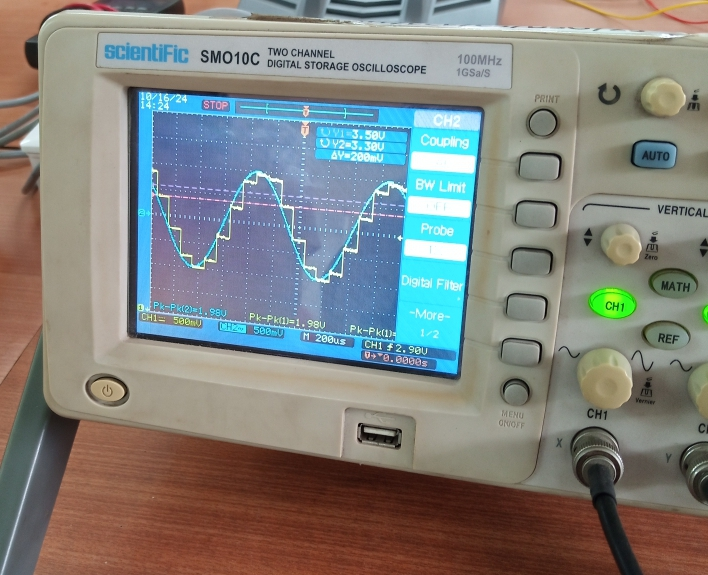
\includegraphics[width=\textwidth]{T1_D10.jpeg}
\caption{Sample and hold with duty cycle=10\%}
\label{fig:T1_D10}
\end{figure}

\begin{figure}[!ht]
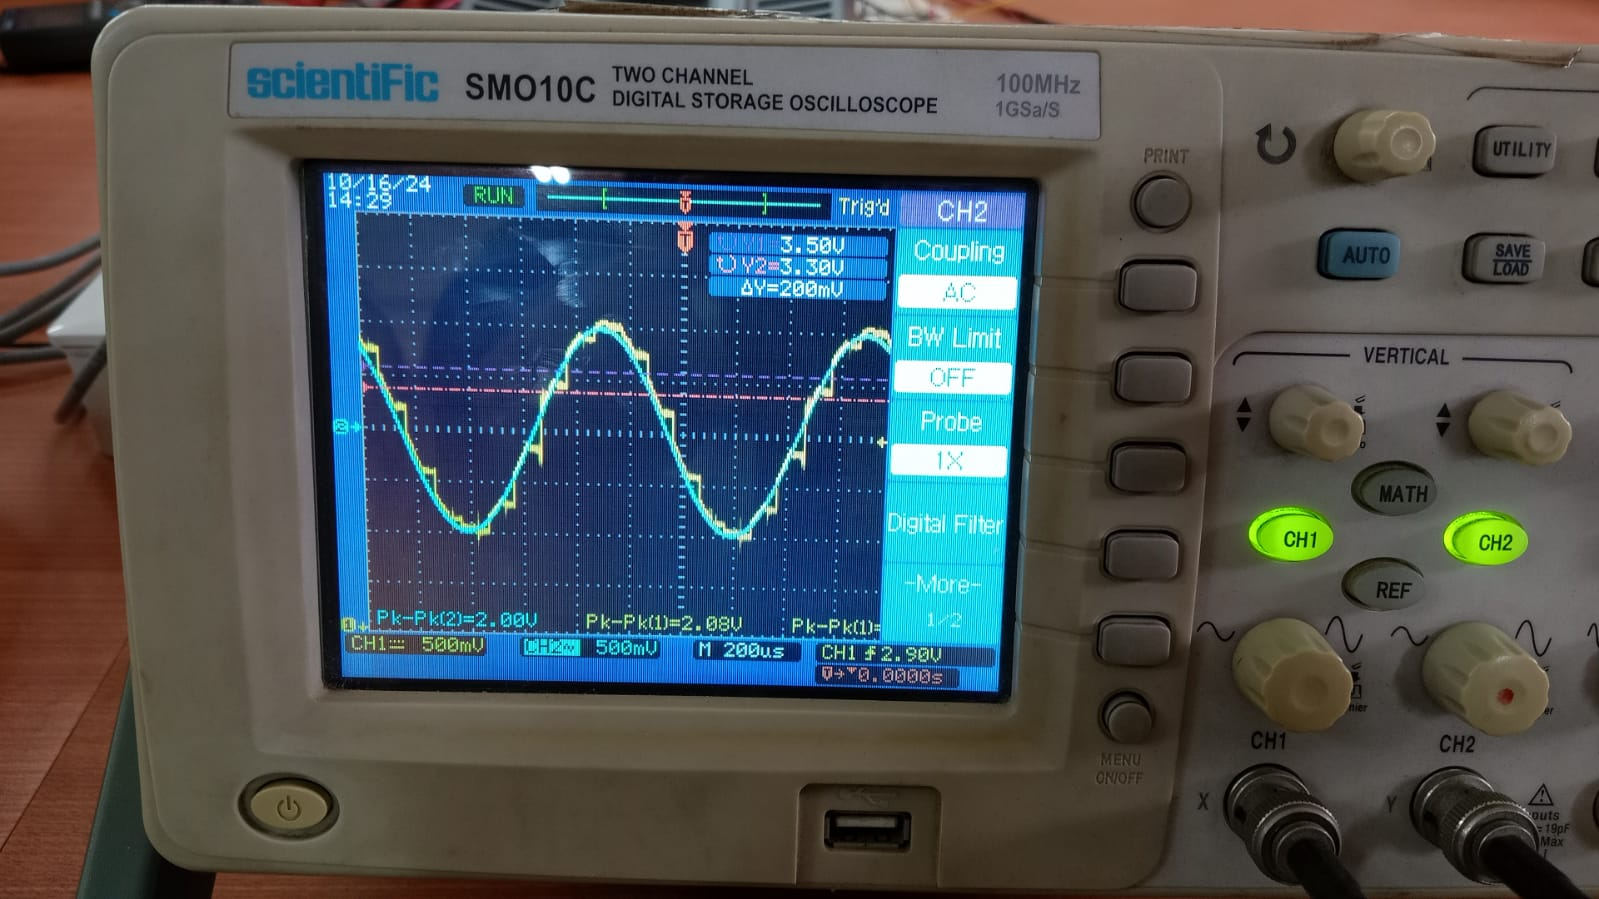
\includegraphics[width=\textwidth]{T1_D50.jpeg}
\caption{Sample and hold with duty cycle=50\%}
\label{fig:T1_D50}
\end{figure}

\begin{figure}[!ht]
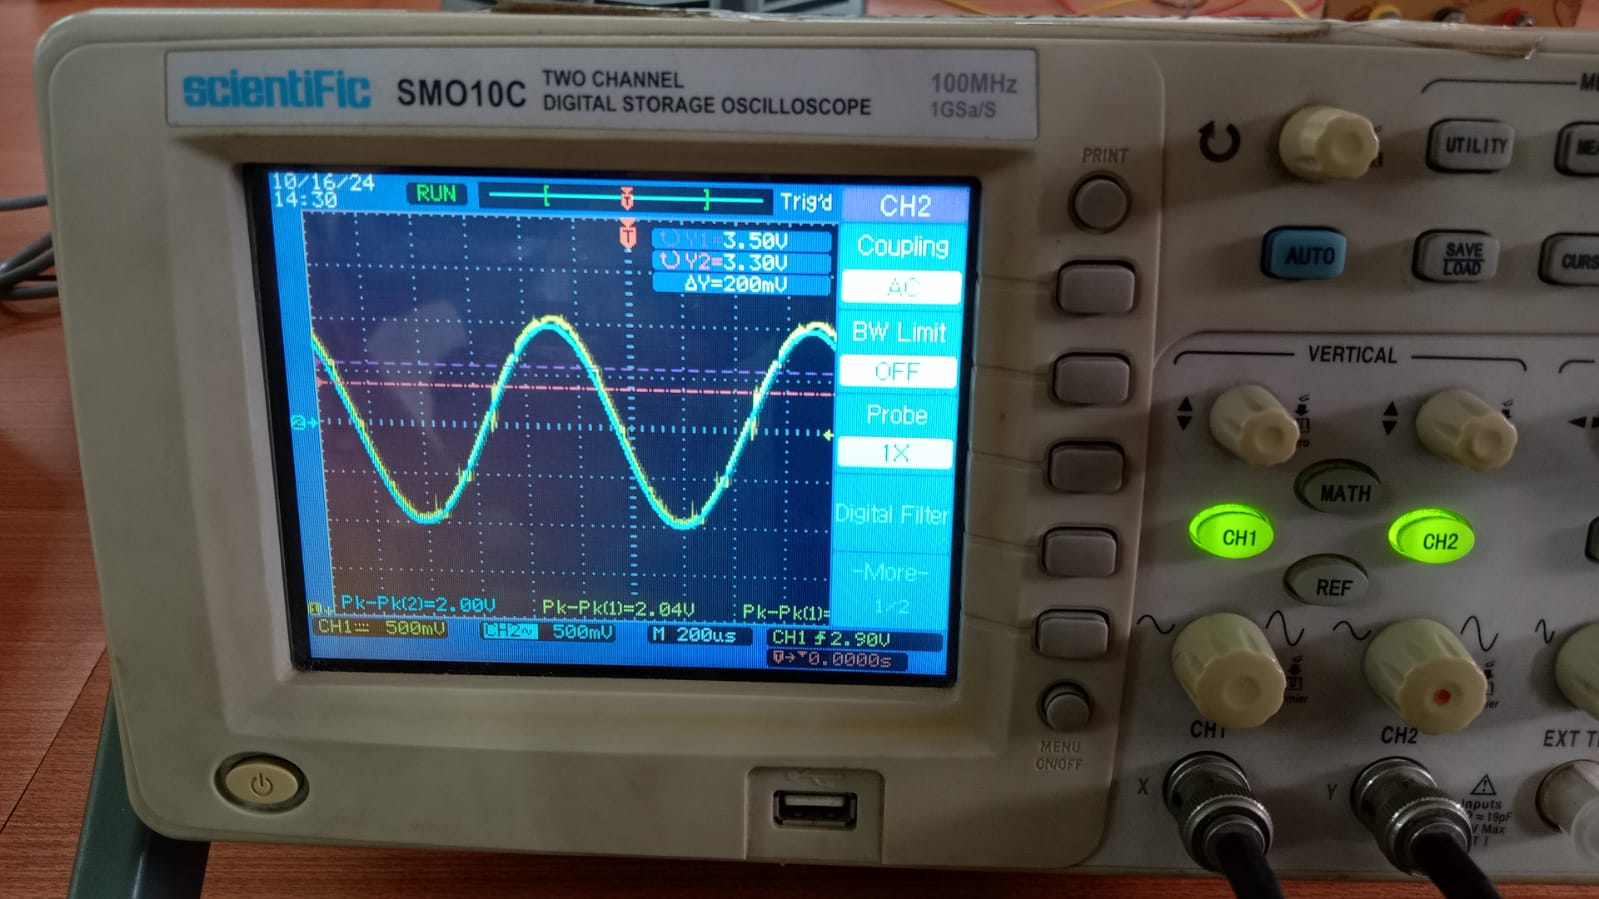
\includegraphics[width=\textwidth]{T1_D80.jpeg}
\caption{Sample and hold with duty cycle=80\%}
\label{fig:T1_D80}
\end{figure}

\begin{figure}[!ht]
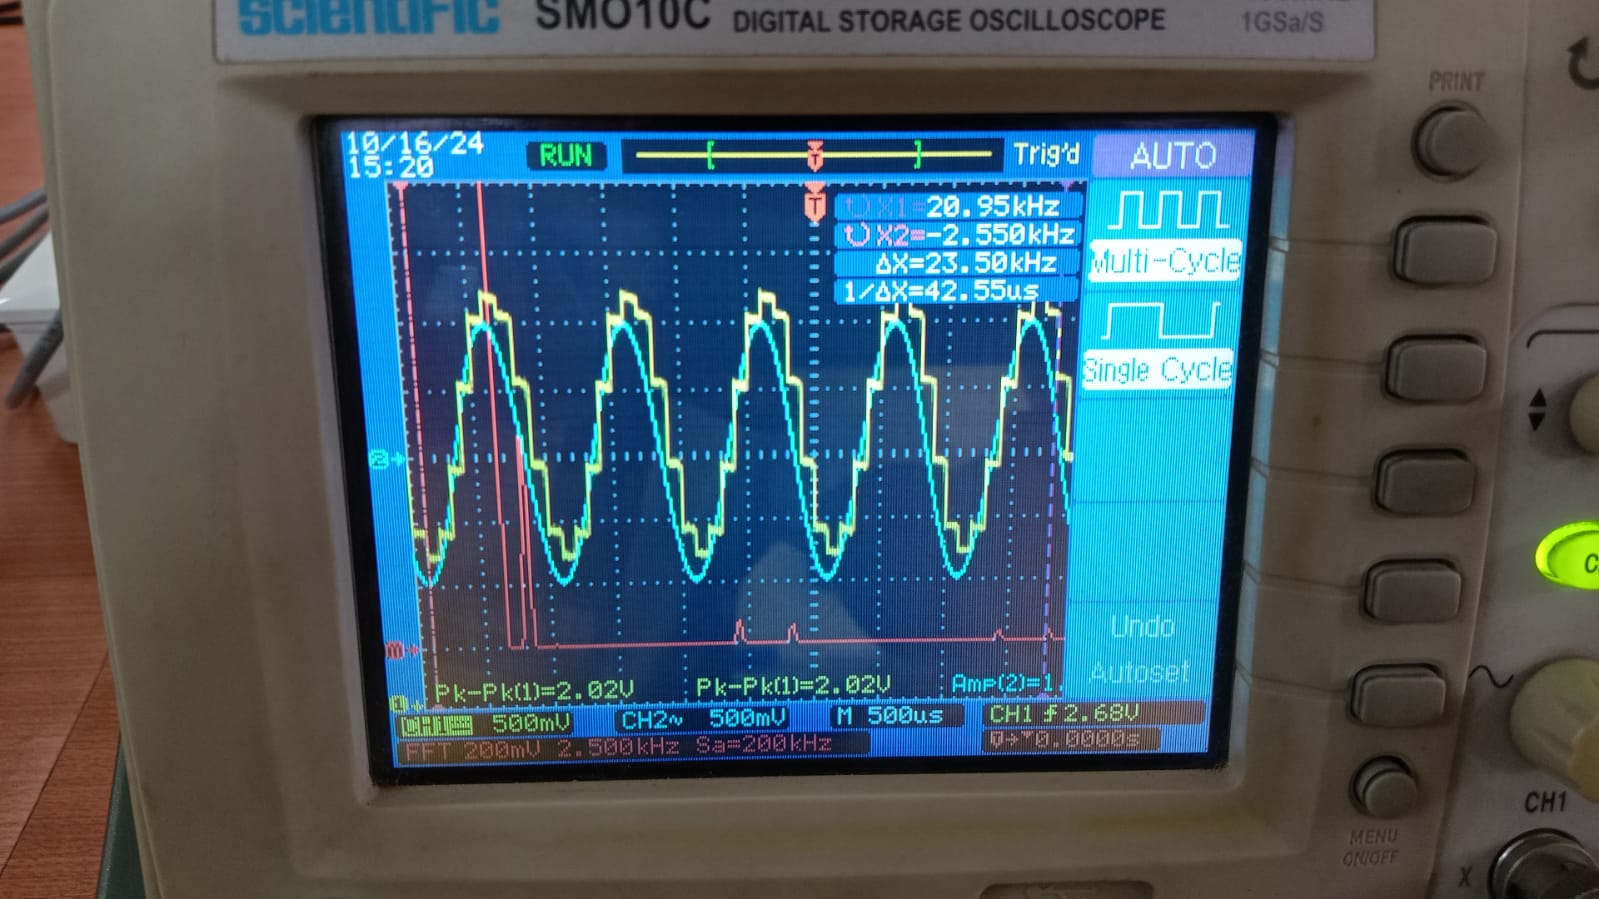
\includegraphics[width=\textwidth]{FFT1.jpeg}
\caption{FFT of the sample and hold signal for D=10\%} 
\label{fig:FFT1}
\end{figure}
\clearpage
\subsection{Task 2}
\begin{figure}[!ht]
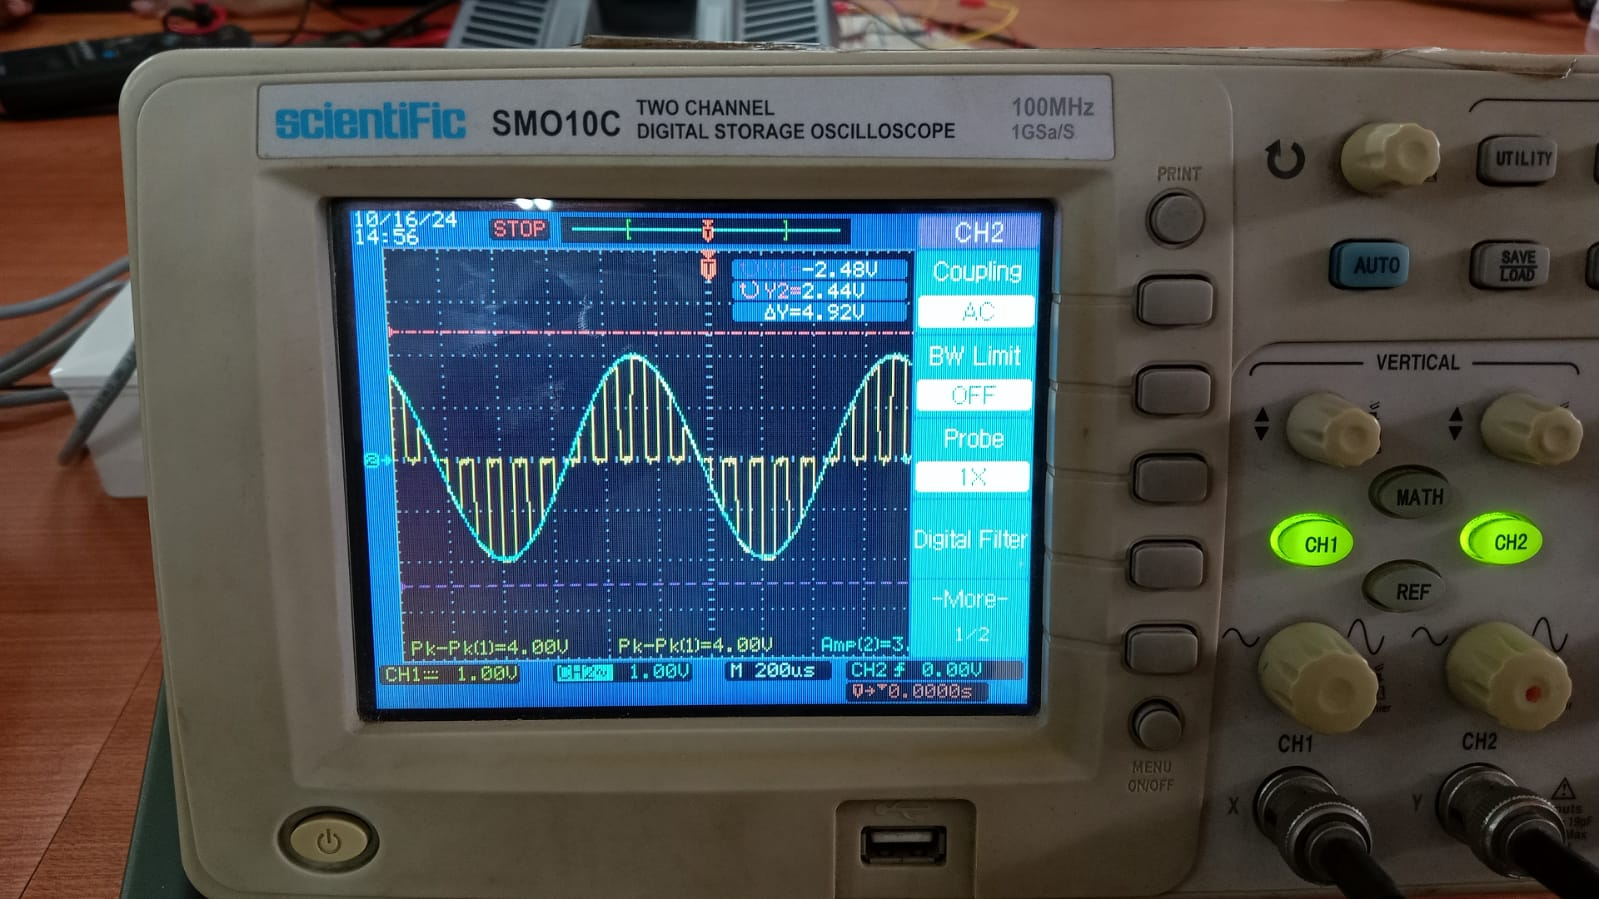
\includegraphics[width=\textwidth]{T2_D50.jpeg}
\caption{Pulse Amplitude Modulated signal with duty cycle=50\%}
\label{fig:T2_D50}
\end{figure}

\begin{figure}[!ht]
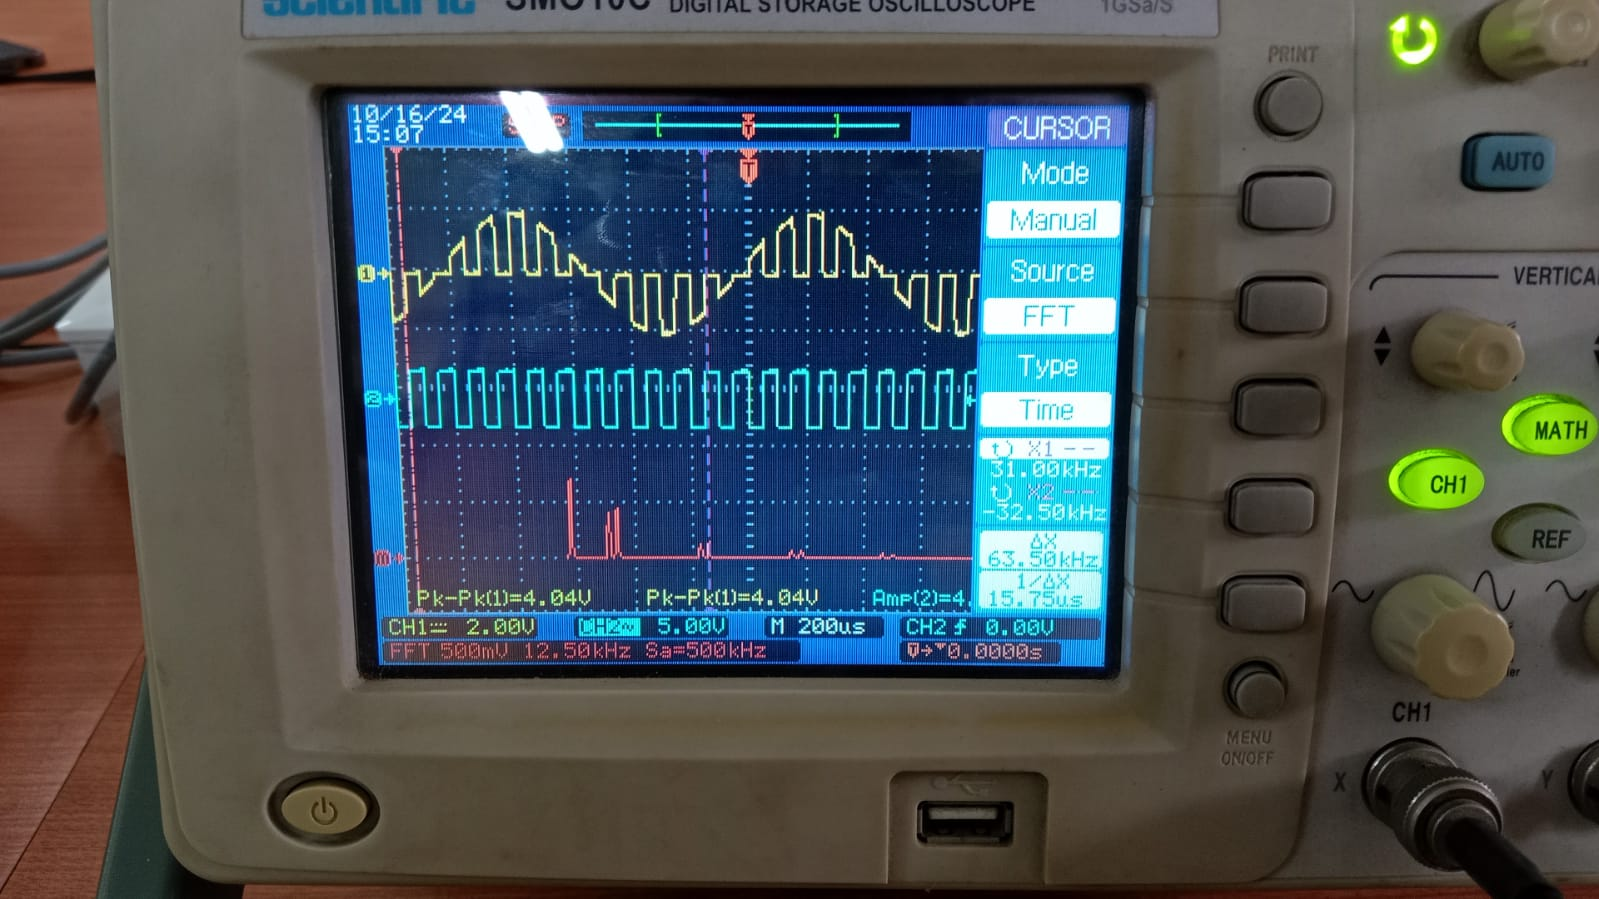
\includegraphics[width=\textwidth]{FFT2.jpeg}
\caption{FFT of the PAM signal for D=50\%}
\label{fig:FFT2}
\end{figure}
\clearpage

\section{Discussion}
\subsection{Samyak Sheersh, 22EC30045}
\begin{enumerate}
  \item As we increased the duty cycle in task 1,  we saw the sample and hold converging on to the signal $m(t)$ see Figures \ref{fig:T1_D10}, \ref{fig:T1_D50} and \ref{fig:T1_D80}. this is expected since a longer duty cycle essentially means that the signal has time to evolve within the aperture time and in the limiting case of $D=100\%$, the circuit just becomes an all pass filter and the output is just the signal $m(t)$
  \item  We found that for the sample and hold signal(i.e Task 1 with $D=10\%$), there were peaks in the FFT at $n\cdot f_s\pm f_m=10n\pm 1$ kHz for $\forall n \in \mathbb{N}$ except for a peak a the original $f_m=1kHz$ and a peak at $f=0$ because of the DC offset.  
  \item We found that for the PAM signal(i.e Task 2), there were peaks in the FFT at $(2n-1)\cdot f_s\pm f_m=10(2n-1)\pm 1$ kHz for $\forall n \in \mathbb{N}$ except for a peak a the original $f_m=1kHz$.  
  \item This difference in the frequencies present in both the signals is also expected since, for the duty cycle at 50\% for Task 2, the pulse becomes a square wave which we know has only odd harmonics, while the pulse with just 10\% duty cycle behaves much more like an impulse and it's Fourier transform is a $sinc$ function i.e the magnitude of the coefficients decays but is non zero for all harmonics, even or odd. 
  \item We also had to add an offset to the signal in Task 1, since a negative $V_{DS}$ was causing distortion in the final signal, which may occur because the reverse flow of current from Source to drain may not be linear in nature and the resulting voltage that we measure may get affected. 
  \item We saw a tradeoff on varying the capacitance. A smaller capacitance would charge up quickly, but it would also discharge quickly and since the total charge on it is less, the voltage reading was also a bit noisy. While larger capacitor took a longer time to charge and discharge, they were less noisy, thus we selected $C=220 pF$ instead of something like $20pF$.
\end{enumerate}
\end{document}

